\chapter{Background and Related Works}
\label{cha:embed}

\section{Neural Probabilistic Language Model}

\com{all quantities have to be defined and described before they are used!!!!!!!!!!}

\com{Please start first with a simple 3-layer neural network as in https://en.wikipedia.org/wiki/Artificial\_neural\_network .You could also use the graphics. Then describe the neural probabilistic language model}

This section will introduce a \emph{neural probabilistic language model} proposed by \cite{BengioDucharmeEtAl2003}. This is one of the first models using word embeddings. So what is a \emph{word embedding}? Generally speaking, for any word $w\in D$ in the dictionary $D$, one can specify a real-valued vector $v(w)\in \mathbb{R}^m$ of fixed length $m$, $v(w)$ called the word embedding of $w$, and $m$ is the length of the word embedding. Note that the $D$ usually contains 10.000 to one million words, whereas the size of the embedding vector is usually in the range of 50 to 1000. A further understanding about the word embeddings will be explained in the next section. 

Since it is a neural probabilistic language model, it is obvious to use an neural network. Figure \ref{fig:neural4} shows the structure of the neural network. It includes four layers: The \emph{Input layer}, the \emph{Projection layer}, the \emph{Hidden layer}  and the \emph{Outputlayer}. $W$ and $U$ are respectively the weight matrix between projection layer and hidden layer and the weight matrix between hidden layer and output layer, \textbf{p} and \textbf{q} are the offset vectors of respectively the hidden layer and the output layer. Further details of word embeddings will be explained in the next section. \com{A neural network defines a mapping between some input and output. Anways specify the input domain and its dimesnion and the output domain! What is the meaning of the input. What is the meaning of the input? }


\begin{figure}[tb]
	\centering
	\fbox{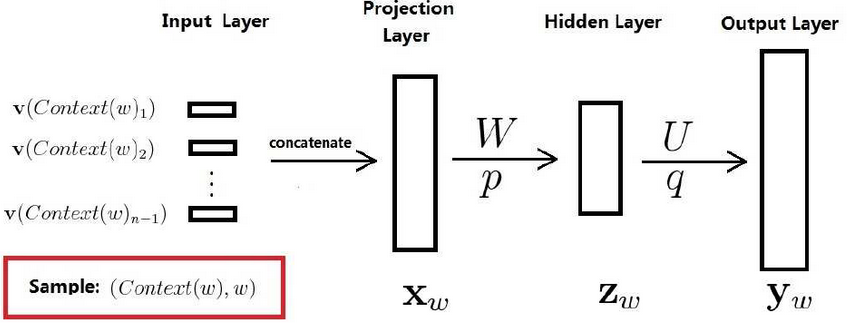
\includegraphics[width=0.7\textwidth]{neural4} }
	\caption{An example of 4 layers neural network.}
	\label{fig:neural4}
\end{figure}
 

\com{Please describe the three-layer network above and then describe the 4-layer network} 
When talking about the above neural network, generally we consider it as a three-layer structure as following Figure \ref{fig:neural3}. But this thesis still use the structure of Figure \ref{fig:neural4}. On the one hand it is easy to describe, on the other hand it is more convenient to do comparison with the network structure in word2vec.

\begin{figure}[!ht]
  \centering
	\fbox{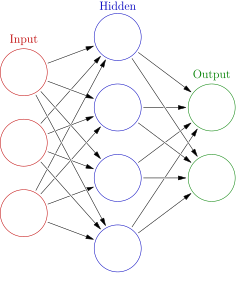
\includegraphics[width=0.5\textwidth]{neural3} }
	\caption{An example of 3 layers neural network}
	\label{fig:neural3}
\end{figure}
\citep{BengioDucharmeEtAl2003} also considers the connection of some neurons from projection layer and some neurons from hidden layer as Figure \ref{fig:bengio}. Thus, there is one more weight matrix. In the numerical experiments, the author found that the introduction of the weight matrix projection layer and output layer can not improve the model effect, but it can reduce the number of training iterations.
\begin{figure}[!ht]
  \centering
	\fbox{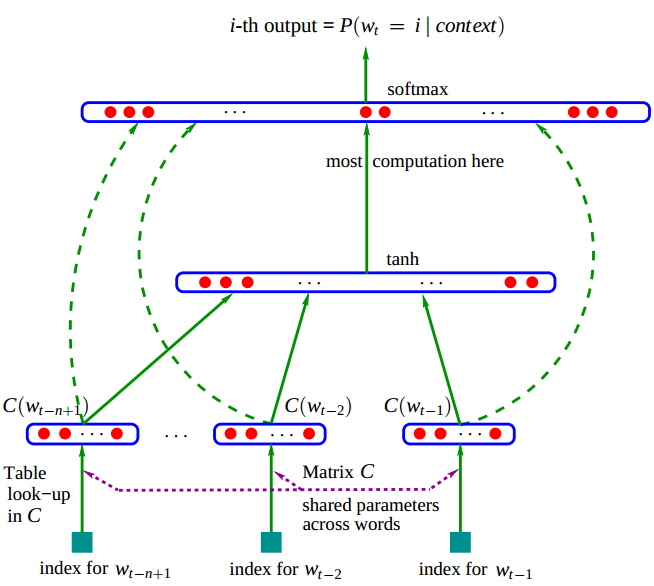
\includegraphics[width=0.7\textwidth]{bengio} }
	\caption{The neural network structure from \citep{BengioDucharmeEtAl2003}}
	\label{fig:bengio}
\end{figure}

We consider a corpus $C$, i.e. a collection of documents with a vocabulary $D$ of words. \com{What do you describe? what is the input, what are the dimensions?} A document $d\in C$ consist of the words $w_1,\ldots,w_t,\ldots,w_T$ with $w_i\in D$. $\ldots$  For any word $w$ in corpus $C$ , assuming $Context(w)$ \com{define!} takes its front $n-1$ words (similar to the n-gram), this binary pair $(Context (w), w)$ is a a training sample.\com{What is the task for which this is used?} So how is the sample $(Context (w), w)$ involved in computing through the neural network? Note that once word corpus $C$ and vector length $m$ is given, the scale of projection layer and the scale of output layer are determined. The former is $(n-1)m$, the latter is $N=|D|$, that is, the size of vocabulary. The size of the hidden layer $n_h$ is the adjustable parameter which can be specified by the user.

Why is the size of the projected layer $(n-1)m$?\com{what is $m$} In fact, the input layer includes $n-1$ words from $Context(w)$, and the vector $\mathbf{x_w}$ from projected layer is built: concatenate $n-1$ input word vectors to be a long vector whose length is $(n-1)m$. With the vector $\mathbf{x_w}$ , the next calculation is clear
\begin{equation}
\left.
\begin{aligned}
\mathbf{z_w} & =  \tanh(W x_w+\mathbf{p}),\\
\mathbf{y_w} & =  U z_w + \mathbf{q}\\
\end{aligned}
\right. \label{eq:neural4}
\end{equation}
where $\tanh$ is the Hyperbolic Tangent Function, used as the \emph{Activation Function} in the hidden layer. In the above formula for a vctor $u=(u_1,\ldots,u_k)$, we define$\tanh(u)=(tanh(u_1,\ldots,tanh(u_k)))$. How about the number of first few words of a given sentence is less than $n-1$? Usually, we can artificially add some filler vectors, and they will also be involved in the training process.

From the above two steps, we get \com{where comes $y_{w,i}$ form? in what set?}  $\mathbf{y_w}=(y_{w,1},y_{w,2},\ldots,y_{w,N})^T$, which is just the vector with the length of $N$ and its components can not represent probabilities. If you want to use $\mathbf{y_w}$'s component $y_ {w,i}$ to represent that the probability of the next word is the $i$-th word when the context is $Context(w)$. Also you need to do a softmax normalization. After normalization, $p(w|Context(w))$ can be expressed as
\begin{equation}\label{eq:softmax}
p(w|Context(w))=\frac{e^{y_{w,i_w}}}{\sum^N_{i=1}e^{y_{w,i}}},
\end{equation}
where $i_w$ represents the index of $w$ in the dictionary $D$. Note that the denominator contains a term $e^{y_{w,i}}$ for every word in the vocabulary.

Formula \ref{eq:softmax} gives the function representation of the probability $p(w|Context(w))$, that is, it gives the function mentioned in the last section $F(w,Context(w),\theta)$. So what is the $\theta$? In conclusion, there are two parts \com{These definitions and dimensions should be given at the beginning!!! Simply state them without questions, describe their meaning and describe the model!}
\begin{itemize}
\item Word vectors: $\mathbf{v}(w)\in \mathbb{R}^m, w\in D$ and the filter vectors
\item Neural network parameters: $W\in \mathbb{R}^{n_h*(n-1)m}, \mathbf{p}\in \mathbb{R}^{n_h}; U \in \mathbb{R}^{N*n_h}, \mathbf{q}\in \mathbb{R}^N$
\end{itemize}
These parameters can be obtained by the training algorithm. On thing needs to be mentioned that, in common machine learning algorithms, the input is already known, however in the above neural probability language model shown as Figure \ref{fig:neural4}, the input $\mathbf{v}(w)$ is not known and also needs to be training.

The next, let's look at the computation of the above model. In the above neural network, the scales of the projection layer, the hidden layer and the output layer are respectively $(n-1)m$, $n_h$, $N$, let's look at the parameters involved:\com{These quatities have to be defined at the first usage of the associated objects}}
\begin{enumerate}
\item $n$ is the number of words contained in the context of a word, usually no more than 5
\item $m$ is the length of word vector, usually the magnitude of $10^1\sim10^3$
\item $n_h$ is specified by the user, usually not too big, like the magnitude of $10^2$
\item $N$ is the size of corpus vocabulary , related with the corpus, usually the magnitude of $10^4$ to $10^6$  
\end{enumerate}
Recombination with \ref{eq:neural4} and \ref{eq:softmax}, it is not difficult to find that, the computing of entire model is mainly about the matrix-vector operations between the hidden layer and the output layer and the softmax normalization in the output layer. Therefore, many of subsequent related works are about optimization for this part, including the the work of word2vec. 

Comparison with n-gram models,\com{What is an n-gram model? Has to be defined!} the neural probabilistic language model mainly has the following two advantages:

\paragraph{Similarity between words can be reflected in the word vectors.}

If in an (English) corpus, $S_1$ = \lq\lq A dog is running in the room\rq\rq\ appears 10000 times, and $S_2$ = \lq\lq A cat is running in the room\rq\rq\ only appears once. According to the n-gram model, $p(S_1)$ will certainly be much greater than $p(S_2)$.\com{Where are $p(S_i)$ defined????} Note that the only difference between $S_1$ and $S_2$ is the \lq\lq dog\rq\rq\ and \lq\lq cat\rq\rq\ , but these two words play the same role either semantically or grammatically, so $p(S_1)$ and $p(S_2)$ should be very close.

However, the probabilities $p(S_1)$ and $p(S_2)$ calculated by the neural network are approximately equal. The reason is that: 
\begin{enumerate}
\item In the neural network probabilistic language model, there is an assumption that the \lq\lq similar \rq\rq\ words should have similar vectors \com{This is a consequence of its definition and not an assumption}
\item The probability function on the word vectors is smooth, that is there is only very small influence for the probability when word vector change a little.\com{This is not true in general, the changes may be drastic! Elaborate the argument!} 
\end{enumerate}
As a result, for the following sentences
\begin{labeling}{alligator}
\item [\tab A dog is running in the room] 
\item [\tab A cat is running in the room]
\item [\tab The cat is running in a room] 
\item [\tab A dog is walking in a bedroom] 
\item [\tab The dog was walking in the room] 
\item [\tab \tab ...] 
\end{labeling}
anyone appears in the corpus, the probabilities of other sentences will increase accordingly.
\paragraph{Models based on the word vector have smoothing already} \com{What does that mean? What is smoothing?}
 (from \ref{eq:softmax}, we can know $p(w|Context(w))\in(0,1)$ can not be $0$), no longer need to carry the additional processing like n-gram model.


Finally, let's look back and think about what kind of role the word vector plays in the neural probability model. When training, it is just the auxiliary parameter used to construct the objective function; after the training, it seems just a by-product of the language model. However, this by-product can not be underestimated, the next section will be further elaborate its usefulness.
%--------------------------------------------------------------------------------------------------------------------------------%
\section{Understanding of the Word Embedding}
In NLP tasks, we will use machine learning algorithms to deal with natural language, but the machine can not directly understand human language, so the first thing is to transform the language to the mathematical form. How can we do such thing? Word vector provides a solution.\\

One of the easiest word vector is one-hot representation, which is to use a long vector to represent a word, the vector's length is  $N$, the size of dictionary $D$. It only has one component which is 1, and the other components are all 0s. The position of 1 corresponds to the index of the word in dictionary. But this word vector representation has some disadvantages, such as troubled by the huge dimensionality, especially when it is applied to deep learning scenes; another thing, it can not describe the similarity between words very well. Another word vector is Distributed Representation, it was firstly proposed by \cite{williams1986learning}, which can overcome the above drawbacks from one-hot representation. The basic idea is to train the particular language to map each word into a short vector of fixed length (here \lq\lq short\rq\rq\ is respected to \lq\lq long\rq\rq\ in one-hot representation). All of these vectors constitute a vector space, and each can be regarded as a a point in the vector space. After introducing the \lq\lq distance\rq\rq in this space , it is possible to judge the similarity between words (morphology and syntax) according to the distance. Actually, word2vec uses this Distributed Representation for word vector.\\

Why is it called Distributed Representation? For one-hot representation, there is only one non-zero vector component, which is very concentrated. For Distributed Representation, vectors have a lot of non-zero components, relatively dispersed. It distributes the information of the word into many components.

Suppose that there are $a$ different points distributed on the two-dimensional plane. For a given point, the task is to find another point closest to this point in the plane. How can we do it? Firstly, establish a Cartesian coordinate system. Based on this coordinate system, each point on which uniquely corresponds to a coordinate $(x, y)$; and then introduce the Euclidean distance; finally calculate the distance between this point and other $a-1$ points, from which the point with the minimum distance is the one we are looking for. In the above example, the role of the coordinates $(x, y)$ is equivalent to the word vector. It is used to mathematically quantify a point on a plane. After the coordinate system is set up, it is very easy to get the coordinate of a point. However, for NLP tasks, to get the word vector is more complex, and the word vector is not unique, which depends on the quality of the training data, training algorithm and other factors.\com{What does this trivial stuff tell us?}

A good word vector is valuable, for example, Ronan Collobert's team makes use of the word vector from software package SENNA (\citep{CollobertWestonEtAl2011}) to do part-ofspeech tagging, chunking into phrases, named entity recognition and semantic role labeling, and achieves good results. Google's Tomas Mikolov team has developed an automatic generation technology for dictionary and glossary, which is able to convert one language into another language. The relation collection between words in each language, that is \lq\lq language space\rq\rq\ , can be characterized as a set of vectors in the mathematical sense.  As long as the mapping and translation of a vector space to another vector space are realized, language translation can be realized. This technique has very good performance for translation between English and Spanish, with the accuracy rate up to $90\%$. 

\section{The model of Collobert and Weston}

\cite{CollobertWeston2008} original main purpose is not to generate a good word vectors, or even do not want to train the language model, but to use this word vectors to complete several tasks from natural language processing, such as speech tagging, named entity recognition, phrase recognition, semantic role labeling, and so on (\citep{CollobertWeston2008} and \citep{CollobertWestonEtAl2011}). Due to the different purpose, their training method is also different and special. They do not use language model's idea like optimizing the probability $P( w_t| w_1, w_2, ... , w_{t - 1})$, but directly use the score $f( w_{t - n + 1}, ... , w_{t - 1}, w_t)$ \com{what is f()} to determine if the sentence is reasonable and normal; low score illustrates the sentence is not reasonable; if you put a few words randomly together, it would be certainly a negative score. The score is just about high or low, not business with probabilities.\com{the score is just a number, the larger the better. Negative / positive is not important. Please write down the equations of the model.} 

With the above assumption, Collobert and Weston used the pair-wise method to train the word vectors. Specifically, it is to minimize the following objective function.\com{you have to define $f$. What is input, what is output?}
$$\sum_{x\in X}\sum_{w\in D}max\{0,1-f(x),f(x^{(w)})\}$$
$X$ is the set of all consecutive $n$-length phrases, $D$ is the entire dictionary. The first summation enumerates all $n$-length phrases from the training set, and each of them positive sample. The second summation for dictionary is to build negative samples. $x(w)$ means the phrase $x$ replacing the middle word to the word $w$. In most cases, replacing the middle of the word in a normal phrase, the new phrase is certainly not the normal phrase, which is a good method to build negative sample (in most cases they are negative samples, only in rare cases the normal phrases are considered as negative samples but they would not affect the final result). \\

The structure of $f$ is almost save as the network structure from \citep{BengioDucharmeEtAl2003}. The same thing is connecting $n$ word vectors together to get a long vector and passing through one layer (a matrix multiplication) to get the hidden layer. The difference is that Collobert and Weston output layer has only one node representing the score, rather than Bengio's $|V|$ nodes.\com{What is $V$?} Doing so greatly reduced the computational complexity. Of course, Collobert and Weston do not want to make a real language model, but just use some idea from the language model to assist them to complete other tasks in NLP.\com{The idea of the first paper was to get a language model!} 

Specifically, they give two different neural network structures window approach and sentence approach, shown as Figure \ref{fig:cw1} and Figure \ref{fig:cw2} respectively.\com{These models are for the subsequent NLP-tasks. Use a figure from \citep{CollobertWeston2008} } Window approach is a feedforward neural network including a linear layer, HardTanh layer. Its input is  the vector concatenated by  all word vectors within the current word window including itself. Window approach is able to deal with most of natural language processing tasks, but has very poor performance on SRL taks. There, they proposed sentence approach to solve such problem. It is convolutional neural network structure. Apart from the linear layer and HardTanh layer, it has another convolutional layer and Max layer. 

\begin{figure}[H]
\centering
\begin{minipage}{.5\textwidth}
 
	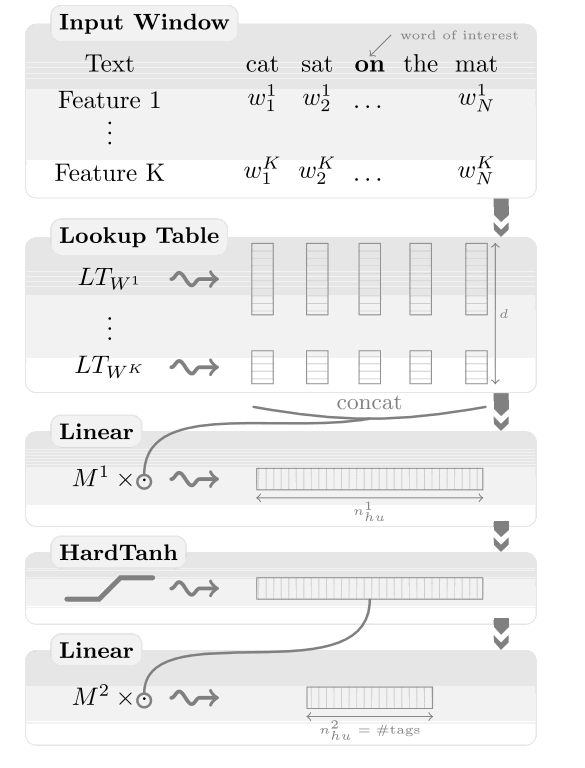
\includegraphics[width=0.9\textwidth]{cw1} 
	\caption{window approach(\cite{CollobertWestonEtAl2011})}
	\label{fig:cw1}
\end{minipage}%
\begin{minipage}{.5\textwidth}
  
	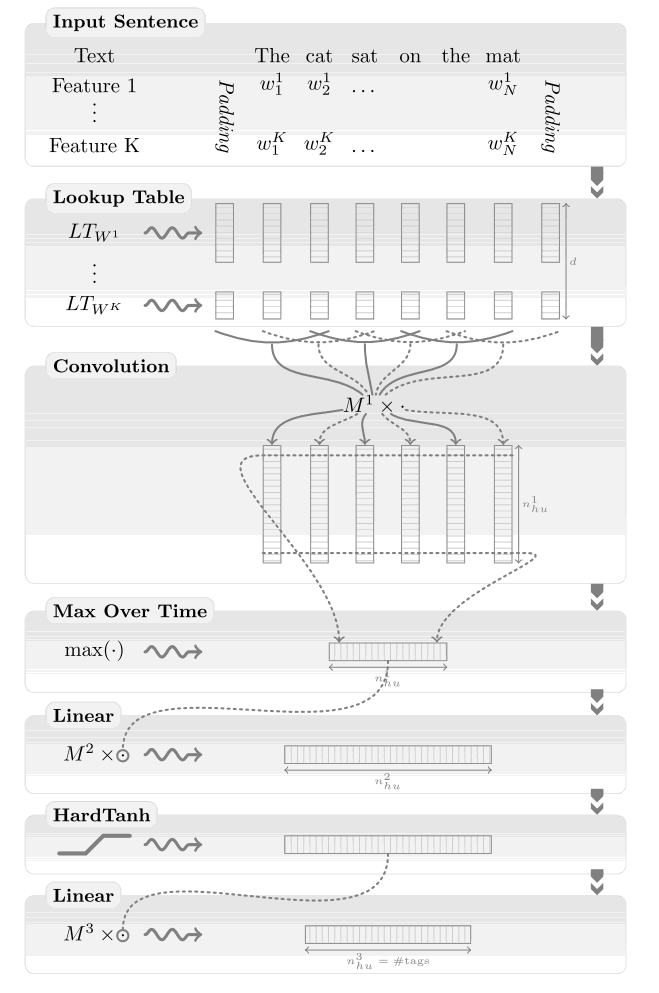
\includegraphics[width=0.85\textwidth]{cw2}
	\caption{sentence approach (\citep{CollobertWestonEtAl2011})}
	\label{fig:cw2}
\end{minipage}
\end{figure}

In the experiment the size of window $n$ is 11 and the size of dictionary $|V|$ is 130000.\com{Before the Dictionary is denoted by $D$. Unify this. I gave you the advice to specify a notation page, but you did not!} They spent totally seven weeks to train word vectors from the Wikipedia English corpus and Reuters corpus.

\section{Word2Vec}
This section will introduce two important model in word2vec: the \emph{CBOW model} (Continuous Bag-of-Words Model) and the \emph{Skip-gram model} (Continuous Skip-gram Model).\com{What is the task of each model? Please specify at the beginning. } 

The CBOW models aims to predict the current word $w_t$ giving its context, e.g. $Context(w_t)=\left\{w_{t-2},w_{t-1},w_{t+1},w_{t+2}\right\}$. Figure \ref{fig:CBOW} of
\cite{MikolovSutskeverEtAl2013} shows the schematic diagram of the CBOW model.
The Skip-gram model shown in figure \ref{fig:Skip-Gram} has the task to predict the words of the context  $Context(w_t)$ from the known current word  $w_t$. 

If we want to predict word $w_t$ from its context the we can use the 
log-likelihood function of the neural network based language model (\ref{eq:softmax}) \com{$C$ was defined without mathcal}
\begin{equation}
\mathcal{L}=\sum_{w\in\mathcal{C}}\log\ p(w|Context(w)) 
\end{equation}
\com{No proper sentence!!!}
For the objective function Hierarchical Softmax CBOW word2vec model based on optimized also the form (4.1); and for the objective function based on Hierarchical Softmax of Skip-gram model, the optimization of the form
\begin{equation}
\mathcal{L}=\sum_{w\in\mathcal{C}}\log\ p(Context(w)|w), 
\end{equation}
Hence the input of the Skip-gram model consists of the words $w_t$ inside the documents of a corpus $C$. For each word the output consist of context of $w_t$, the set $Context(w_t)$. The words in the input as well as the output are projected on an embedding. The specific feature of the word2vec approach is that two different embeddings are use for the words in the input and words in the output.
Note that the denominator contains a term for every word in the vocabulary. With a vocabulary often larger than 100k words the associated computational effort is prohibitive. Therefore \cite{MikolovSutskeverEtAl2013} propose two important simplifications.
\begin{center}
\begin{figure}[tb]
\centering
\begin{minipage}{.49\textwidth}
 
	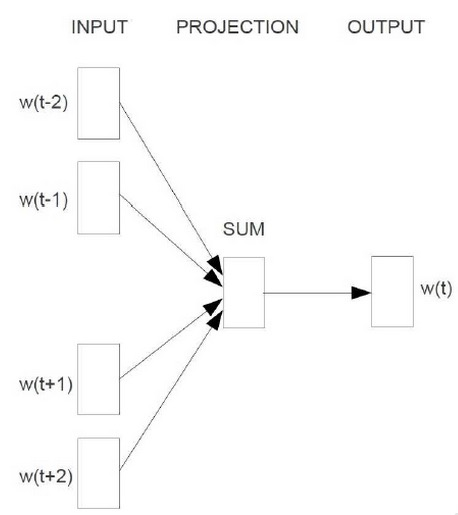
\includegraphics[width=0.9\textwidth]{CBOW} 
	\caption{Structure of the CBOW model predicting the current word from its context words.}
	\label{fig:CBOW}
\end{minipage}%
\hspace{.01\textwidth}
\begin{minipage}{.49\textwidth}
  
	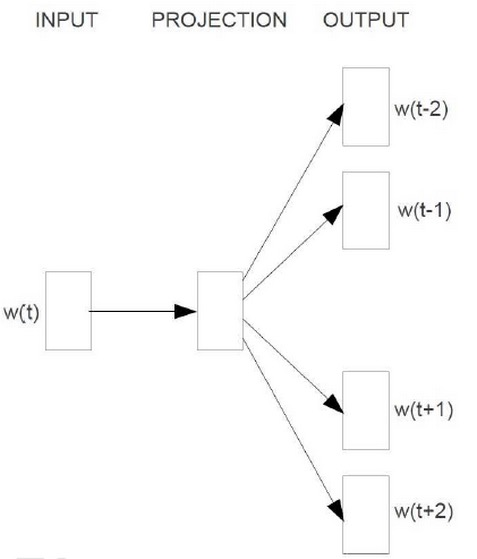
\includegraphics[width=0.85\textwidth]{Skip-Gram}
	\caption{Structure of the Skip-Gram model predicting the context words from the current word. }
	\label{fig:Skip-Gram}
\end{minipage}
\end{figure}
\end{center}


\subsection{Skip-gram model with Hierarchical Softmax}

\subsubsection {Gradient Calculation} 
For Skip-gram model has to predict  its context $Context(w)$ of the words using the current word $w$ as input. \cite{MikolovSutskeverEtAl2013} propose the following the objective function 
\begin{equation}
p(Context(w)|w)=\prod_{u\in Context(w)}p(u|w)
\end{equation}
$p(u|w)$ is the probability of a single output word $u$ given the current word $w$.

\com{I do not understand the following text!!!!! You have to motivate this by some hierarchical splitting example Huffman tree}   
In the above formula $p(u|w)$ in accordance with section describes the Hierarchical Softmax thought, similar to (4.3) written as
$$p(u|w)=\prod_{j = 2}^{l^u}p(d^u_j|\text{v}(w),\theta^u_{j-1}), $$
among them
\begin{equation}
p(d^u_j|\mathbf{v}(w),\theta^u_{j-1})=[\theta(\mathbf{v}(w)^{\mathrm{T}}\theta^u_{j-1})]^{1-d^u_j}\cdot[1-\theta(\mathbf{v}(w)^{\mathrm{T}}\theta^u_{j-1})]^{1-d^u_j}
\end{equation}
The (4.6) followed by generations back, you can get the log-likelihood function (4.2) of the specific expression
\begin{equation}
\mathcal{L}=\sum_{w\in\mathcal{C}}\log\prod_{u\in Context(w)}\prod_{j=2}^{l^u}\{[\theta(\mathbf{v}(w)^{\mathrm{T}}\theta^u_{j-1})]^{1-d^u_j}\cdot[1-\theta(\mathbf{v}(w)^{\mathrm{T}}\theta^u_{j-1})]^{\ d^u_j}\} \\
\ \ \ $$ $$=\sum_{w\in\mathcal{C}}\sum_{u\in Context(w)}\sum_{j=2}^{l^u}\{(1-d^u_j)\cdot\log[\theta(\mathbf{v}(w)^{\mathrm{T}}\theta^u_{j-1})]+d^u_j\cdot\log[1-\theta(\mathbf {v}(w)^{\mathrm{T}}\theta^u_{j-1})]\}.
\end{equation}
Similarly, as in the following gradients of convenience, under the triple summation symbol braces contents of abbreviated as $\mathcal{L}(w,u,j)$, ie
$$\mathcal{L}(w,u,j)=(1-d^u_j)\cdot\log[\theta(\mathbf{v}(w)^{\mathrm{T}}\theta^u_{j-1})]+d^u_j\cdot\log[1-\theta(\mathbf{v}(w)^{\mathrm{T}}\theta^u_{j-1}]. $$
So far, it has been deduced logarithmic likelihood function of expressions like (4.7), which is the objective function Skip-gram model. Then also use stochastic gradient ascent method to optimize the key is to give two types of gradients.
First consider $\mathcal{L}(w,u,j)$ on $\theta^u_{j-1}$ gradient calculation (with the corresponding portion of the model is derived CBOW completely analogous).
$$\partial\frac{\mathcal{L}(w, u, j)}{\partial\theta^u_{j-1}}=\frac{\partial}{\partial\theta^u_{j-1}}\{(1-d^u_j)\cdot\log[\theta(\mathbf{v}(w)^{\mathrm{T}}\theta^u_{j-1})]+d^u_j\cdot\log[\theta(\mathbf{v}(w)^{\mathrm{T}}\theta^u_{j-1})]\}$$
\com{Is this approach exact or an approximation?}

\subsection{Skip-gram with Negative Sampling}

Negative Sampling (NEG) is proposed by \cite{MikolovSutskeverEtAl2013}, which is the simplified version of NCE(Noise Contrastive Estimation)\com{need a reference}. The purpose is to improve the training and the quality of word vectors. In comparison with Hierarchical Softmax, NEG do not use the Huffman tree. Instead, it use Random Negative Sampling, which can improve the performance much.\com{Where is this prooved?}

The details of NCE is a little complex, the essence is to use a known probability density function to estimate an unknown probability density function. In short, assume there is an unknown probability density function $Y$ and a known probability density function $X$, if we get the relationship between $X$ and $Y$, we can obtain $X$ as well.The detail of method reference to [NCE]. 

The objective function is:
\begin{equation}
G=\prod_{w\in\mathcal{C}}\prod_{u\in Context(w)}g(u),
\end{equation}
Here, we want to maximize $\prod_{u\in Context(w)}g(u)$ giving $(w, Context(w)))$,  and $g(u)$ is defined as
$$
g(u)=p(z|w)*\prod_{z\inNEG(u)}p(z|w),
$$
where $NEG(u)$ represents the negative samples\com{what is that?} generated by $u$, the conditional probability\com{the negative samples are not generated by this conditional probability. What is $\theta$?}
$$p(z|w)=
\sigma(\mathbf{v}(w)^{\mathrm{T}}\theta^z) 
$$
It can also be written as one expression
\begin{equation}
p(z|w)=[\sigma(\mathbf{v}(w)^{\mathrm{T}}\theta^z)]^{L^u(z)}\cdot[1-\sigma(\mathbf{v}(w)^{\mathrm{T}}\theta^z)]^{1-L^u(z)}
\end{equation}
where \com{L was the likelihood, choose another letter} $$L^u(z) = \left\{
\begin{aligned}
1, && u = z;\\
0, && u \neq z,\\
\end{aligned}
\right.
$$
And then we use the log of $G$, so the final objective function is 
\begin{align*}
L & =\log\ G=\log \prod_{w\in\mathcal{C}}\prod_{u\in Context(w)} g(u)=\sum_{w\in\mathcal{C}}\sum_{u\in Context(w)} \log\ g(u) \\
& = \sum_{w\in\mathcal{C}}\sum_{u\in Context(w)} \log\left( p(u|w)\prod_{z\in NEG(u)} p(z|w)\right) \\
& = \sum_{w\in\mathcal{C}}\sum_{u\in Context(w)}\left(\log  p(u|w)+ \sum_{z\in NEG(u)} \log\ p(z|w)\right) \\
& = \sum_{w\in\mathcal{C}}\sum_{u\in Context(w)}\sum_{z\in\{u\}\cup NEG(u)} \log\ \{[\sigma(\mathbf{v}(w)^{\mathrm{T}}\theta^z)]^{L^u(z)}\cdot[1-\sigma(\mathbf{v}(w)^{\mathrm{T}}\theta^z)]^{1-L^u(z)}\} \\
& = \sum_{w\in\mathcal{C}}\sum_{u\in Context(w)}\sum_{z\in\{u\}\cup NEG(u)}\{L^u(z)\cdot \log[\sigma(\mathbf{v}(w)^{\mathrm{T}}\theta^z)]+[1-L^u(z)]\cdot\log[1-\sigma(\mathbf{v}(w)^{\mathrm{T}}\theta^z)]\}.
\end{align*}
In order to calculate the gradient more conveniently, we use $L(w,u,z)$ to represent the contents of curly braces as
$$\mathcal{L}(w,u,z)=L^u(z)\cdot \log[\sigma(\mathbf{v}(w)^{\mathrm{T}}\theta^z)]+[1-L^u(z)]\cdot\log[1-\sigma(\mathbf{v}(w)^{\mathrm{T}}\theta^z)]$$
\cite{MikolovSutskeverEtAl2013} use the \textbf{Stochastic gradient ascent method} to minimize $\mathcal{L}(w,u,z)$. The point is to calculate two kinds of gradient. Let's consider the gradient with respect to $\theta^z$ firstly.
\begin{align*}
& \ \ \ \ \frac{\partial\mathcal{L}(w,u,z)}{\partial\theta^z} \\
& =  \frac{\partial}{\partial\theta^z} \{ L^u(z)\cdot \log[\sigma(\mathbf{v}(w)^{\mathrm{T}}\theta^z)]+[1-L^u(z)]\cdot\log[1-\sigma(\mathbf{v}(w)^{\mathrm{T}}\theta^z)] \} \\
& =  L^u(z)[1-\sigma(\mathbf{v}(w)^{\mathrm{T}}\theta^z)]\mathbf{v}(w) - [1-L^u(z)]\sigma(\mathbf{v}(w)^{\mathrm{T}}\theta^z)\mathbf{v}(w) \\
& = \{L^u(z)[1-\sigma(\mathbf{v}(w)^{\mathrm{T}}\theta^z)]-[1-L^u(z)]\sigma(\mathbf{v}(w)^{\mathrm{T}}\theta^z)\}\mathbf{v}(w) \\
& = [L^u(z)-\sigma(\mathbf{v}(w)^{\mathrm{T}}\theta^z)] \mathbf{v}(w).
\end{align*}
Thus, the updating formula of $\theta^z$ can be written as
$$\theta^z:=\theta^z+\eta[L^u(z)-\sigma(\mathbf{v}(w)^{\mathrm{T}}\theta^z)]\mathbf{v}(w).$$
The next, let's consider the gradient of $\mathbf{v}(w)$. Using the symmetry of \textbf{v}(w) and $\theta^z$, we have
$$\frac{\partial\mathcal{L}(w,u,z)}{\partial\mathbf{v}(w)} = [L^u(z)-\sigma(\mathbf{v}(w)^{\mathrm{T}}\theta^z)]\theta^z,$$
Thus, the updating formula of $\mathbf{v}(u)$ can be written as 
$$\mathbf{v}(w):=\mathbf{v}(w)+\eta\sum_{z\in\{u\}\cup NEG\{u\}}\frac{\partial\mathcal{L}(w,u,z)}{\partial\mathbf{v}(w)}$$
$$=\mathbf{v}(w)+\eta\sum_{z\in\{u\}\cup NEG\{u\}}[L^u(z)-\sigma(\mathbf{v}(w)^{\mathrm{T}}\theta^z)]\theta^z.$$

\section{Huang's Model}


The work of \cite{HuangSocherEtAl2012} is based on the model of \cite{CollobertWeston2008}. They try to make embedding vectors with richer semantic information. They had two major innovations to accomplish this goal : The first innovation is using global information from the whole text to assist local information, the second innovation is using the multiple word vectors to represent polysemy. 

Huang thinks \cite{CollobertWeston2008} use only "local context". In the process of training vectors, they used only 10 words as the context for each word, counting the center word itself, there are totally 11 words' information. 
This local information can not fully exploit the semantic information of the center word. Huang used their neural network directly to compute a score as the "local score". 

And then Huang proposed a "global information", which is somewhat similar to the traditional bag of words model. Bag of words is about accumulating One-hot Representation from all the words of the article together to form a vector (like all the words thrown in a bag), which is used to represent the article. Huang's global information used the average weighted vectors from all words in the article (weight is word's idf), which is considered the semantic of the article. 
He connected such semantic vector of the article (global information) 
with the current word's vector (local information) to form a new vector with double size as an input, and then used the C$\&$W's network to calculate the score. Figure [huang] shows such structure.
With the "local score" from original C$\&$W approach and "Global score" from improving method based on the C$\&$W approach, Huang directly add two scores as the final score. The final score would be optimized by the pair-wise target function from C$\&$W. Huang found his model can capture better semantic information. \\

\begin{figure}[!ht]
  \centering
	\fbox{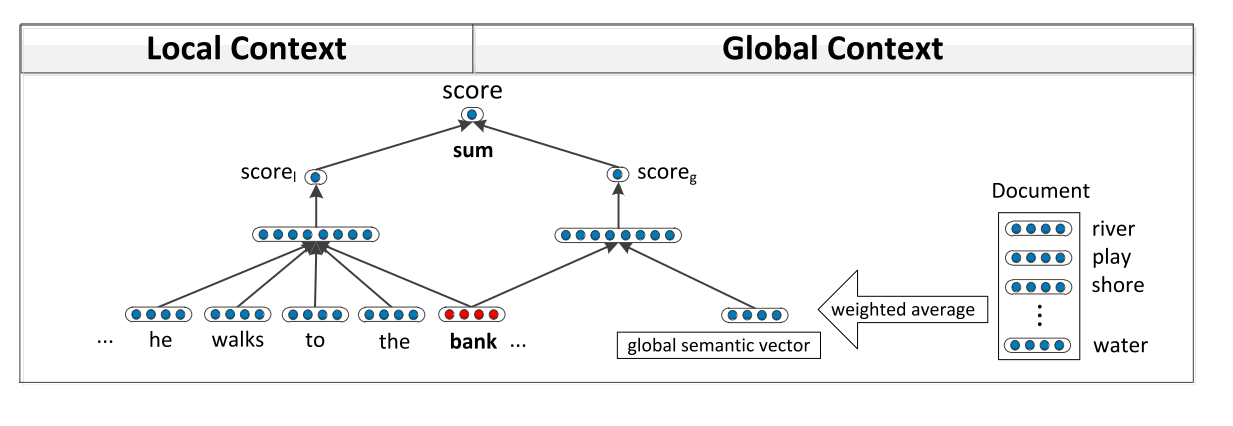
\includegraphics[width=0.9\textwidth]{huang} }
	\caption{The network structure from \citep{huang2012improving}}
	\label{fig:huang}
\end{figure}


The second contribution of this paper is to represent polysemy using multiple embeddings for a single word. \citep{bengio2003neural} also mentioned that this would be an very important issue, but he was still looking for a solution, now Huang gives an idea. For each center word, he took 10 nearest context words and calculated the weighted average of the embeddings of these 10 word vectors (idf weights) as the context vector. Huang used all context vectors to do a k-means clustering. The number of clusters \com{where does he get them??}. He relabel  each word  based on the clustering results (different classes of the same words would be considered as different words to process)\com{How was this exactly done?}. Finally he re-trained the word vectors. Table~\ref{tab:huang} gives some examples from his model's results.\\

\begin{table}[tb]
\begin{center}
\caption{Senses computed with Huang's network and their nearest neighbors.} 
\label{tab:huang}
\vspace{2mm}
 \begin{tabular}{|l|l|}
  \hline
  Center Word &Nearest Neighbors \\
  \hline  
  bank$\_$1 & corporation, insurance, company\\
  \hline
  bank$\_$2 & shore, coast, direction\\
  \hline
  star$\_$1 & movie, film, radio\\
  \hline
  star$\_$2 & galaxy, planet, moon\\
  \hline
  cell$\_$1 & telephone, smart, phone\\
  \hline
  cell$\_$2 & pathology, molecular, physiology\\
  \hline
  left$\_$1 & close, leave, live\\
  \hline
  left$\_$2 & top, round, right\\
  \hline
 \end{tabular}
\end{center}
\end{table}

\section{EM-Algorithm based method}


\cite{TianDaiEtAl2014} proposed an approach based on the EM-algorithm from . This method is the extension of the normal skip-gram model. They still use each center word to predict several context words. The difference is that each center word can have several senses with different probabilities. The probability should represent the relative frequency of the sense in the corpus. For example, considering $bank_1$ in the sense of "side of the river" and $bank_2$ meaning "financial institution". Usually $bank_1$ will have a smaller probability and $bank_2$. We can say in the corpus, in most sentences of the corpus the word "bank" means "financial institution" and in other fewer cases it means "side of the river". 

\paragraph{Objective Function}\

Considering $w_I$ as the input word and $w_O$ as the output word, $(w_I,w_O)$ is a data sample. The input word $w_I$ have $N_{w_I}$ prototypes, and it appears in its $h_{w_I}$-th prototype, i.e., $h_{w_I}\in \{1,..,N_{w_I}\}$ [] The prediction $P(w_O|w_I)$ is like the following formula
$$p(w_O|w_I)=\sum^{N_{w_I}}_{i=1}P(w_O|h_{w_I}=i,w_I)P(h_{w_I}=i|w_I)=\sum^{N_{w_I}}_{i=1}\frac{exp(U^{\mathrm{T}}_{w_O}V_{w_I,i})}{\sum_{w\in W exp(U^\mathrm{T}_w V_{w_I,i})}}P(h_{w_I}=i|w_I)$$
where $V_{w_I,i}\in R^d$ refers to the d-dimensional "input" embedding vector of $w_I$'s $i$-th prototype and $U_{w_O}\in R^d$ represents the "output" embedding vectors of $w_O$. Specifically, they use the Hierarchical Softmax Tree function to approximate the probability calculation. 

\begin{table}[tb]
	\begin{center}
		\caption{Word senses computed by \citeauthor{TianDaiEtAl2014}}
		\label{tab:tian}
		\vspace{2mm}
		\begin{tabular}{|l|l|l|}
			\hline
			word & Prior Probability & Most Similar Words \\
			\hline  
			apple$\_$1 & 0.82 & strawberry, cherry, blueberry\\
			\hline
			apple$\_$2 & 0.17 & iphone, macintosh, microsoft\\
			\hline
			bank$\_$1 & 0.15 & river, canal, waterway\\
			\hline
			bank$\_$2 & 0.6 & citibank , jpmorgan, bancorp\\
			\hline
			bank$\_$3 & 0.25 & stock, exchange, banking\\
			\hline
			cell$\_$1 & 0.09 & phones cellphones, mobile\\
			\hline
			cell$\_$2 & 0.81 & protein, tissues, lysis\\
			\hline
			cell$\_$3 & 0.01 &locked , escape , handcuffed\\
			\hline
		\end{tabular}
	\end{center}
	
\end{table}

\paragraph{Algorithm Description}\ 

Particularly for the input word $w$, they put all samples ($w$ as the input word) together like $\{(w, w_1), (w, w_2), (w, w_3) ... (w, w_n)\}$ as a group. Each group is based on the input word. So the whole training set can be separated as several groups. For the group mentioned above, one can assume the input word $w$ has $m$ vectors ($m$ senses), each with the probability $p_j (1 \leq j \leq m)$. And each output word $w_i (1 \leq i\leq n)$ has only one vector. 

 In the training process, for each iteration, they fetch only part of the whole training set and then split it into several groups based on the input word. In each E-step, for the group mentioned above, they used soft label $y_{i,j}$ to represent the probability of input word in sample $(w,w_i)$ assigned to the $j$-th sense. The calculating of $y_{i,j}$ is based on the value of sense probability and sense vectors. After calculating each $y_{i,j}$ in each data group, in the M-step, they use $y_{i,j}$ to update sense probabilities and sense vectors from input word, and the word vectors from output word. Table~\ref{tab:tian} lists some results from this model.

\section{A Method to Determine the Number of Senses}
\cite{NeelakantanShankarEtAl2015} \com{Write a paragraph on this}
